This section mostly follows \cite{dependability}, including some tables, which is available online.

Computer systems can be evaluated according to
\begin{compactitem}
 \item functionality
 \item usability
 \item performance
 \item cost
 \item dependability
\end{compactitem}

\textbf{Dependability} means to deliver service to a user that can justifiably be trusted.
The user is another system (physical or human) that interacts with the former at the service interface.
The \textbf{function} of a system is what the system is intended to do as described by its functional specification.
Correct service is delivered when the service implements the specification.

A systematic exposition of the concepts of dependability consists of three parts: the attributes of dependability, their threats, and means to achieve dependability.
An overview is given in Fig.~\ref{fig:concepts_dep}.

\begin{figure}
\centering
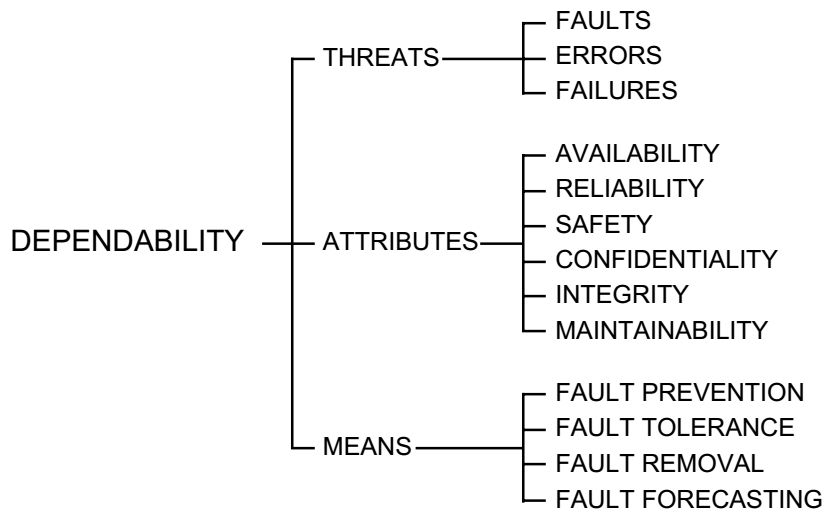
\includegraphics[width=0.7\linewidth]{concepts_dep}
\caption{Concepts Related to Dependability}
\label{fig:concepts_dep}
\end{figure}

\section{Attributes}

\subsection{Definitions}

\textbf{Availability} means the readiness for correct service.
This includes two subaspects: the functionality has to \textbf{exist} and be realized \textbf{correctly}, i.e., according to its specification.

\textbf{Reliability} means the continuity of correct service.
This is similar to availability but emphasizes that the service not only exists but exist without downtime or intermittent failures.

\textbf{Safety} means the absence of catastrophic consequences on the user(s) and the environment.
Often safety involves interpreting signals received from and sending signals to external devices that operate in the real world, e.g., the cameras and the engine of the car.
This introduces additional uncertainty (not to mention the other cars and pedestrians) that can be difficult to anticipate in the specification.

\textbf{Security} means the availability for authorized users only.
This includes protection against any malicious influenced from the outside, i.e., any kind of attack or hacking.
This includes all defenses against hacking.\footnote{\cite{dependability} calls a related property \emph{integrity}, and then defines security as the combination of integrity and confidentiality.}

\textbf{Confidentiality} means the absence of unauthorized disclosure of information.
This includes the security of all private data including any intermediate results of computation such as passwords or keys.

\textbf{Maintainability} means the ability to undergo repairs and modifications.
This includes all necessary changes needed during long-term deployment.

\subsection{Incomplete Specifications}

Often the attributes are not or only implicitly part of the specification of a system.

Availability is usually implicitly required, but details may be omitted.
For example, the acceptable variation of response times may be unspecified.

Reliability is also usually implicit required, but details may be omitted.
For example, the acceptable downtime may be unspecified.

Safety is usually specified well if a potential safety danger is realized.
But it can be easy to foresee all necessary safety requirements.

Security is often forgotten completely or partially.
It is usually difficult to translate the abstract requirement of security into concrete, testable properties.
After all, the first mistake of security is to assume to know what the attacker might do.

Confidentiality is often considered even less then security.

Maintainability is often ignored completely.
That is a typical pitfall for large projects, where realizing any requirement at deploy time may be completely different from realizing it after a year or later.
This is because intermediate changes have messed up the system so much that, e.g., security flaws are not noticed anymore.

\subsection{Imperfect Implementations}

All attributes are very difficult to realize perfectly in implementations.

Availability and reliability often fail.
In addition to plain design or implementation errors, there may be failures in hardware, networks, operating system, external components that were not foreseen by the developer.

Together with correctness, safety is the only property that is at least in principle accessible to a formal definition.
But the resulting problem is undecidable.
So in practice, we have to use to extensive testsmust be established in complex 

Security is very to prove because any proof must make assumptions about what kind of attacks there are.
Attacking a system often requires intentionally violating the specification and supply unanticipated input.

Perfect confidentiality is impossible to realize because all computation leaks some information other than the output: This reaches from runtime and resource use to obscure effects like the development of heat due to CPU activity.

Maintainability is hard to realize because especially inexperienced developers or unskilled managers cannot assess whether a particular design is maintainable.

\section{Threats}

\subsection{Failures}

A system \textbf{failure} is an event that occurs when the delivered service deviates from correct service.
See Fig.~\ref{fig:concepts_fail} for an overview of related concepts.

A \textbf{fault} is the adjudged or hypothesized cause of an error.
A fault is \textbf{active} when it produces an error; otherwise it is \textbf{dormant}.
See Fig.~\ref{fig:concepts_fault} for an overview of related concepts.

An \textbf{error} is that part of the system state that may cause a subsequent failure: a failure occurs when an error reaches the service interface and alters the service.

\begin{figure}
\centering
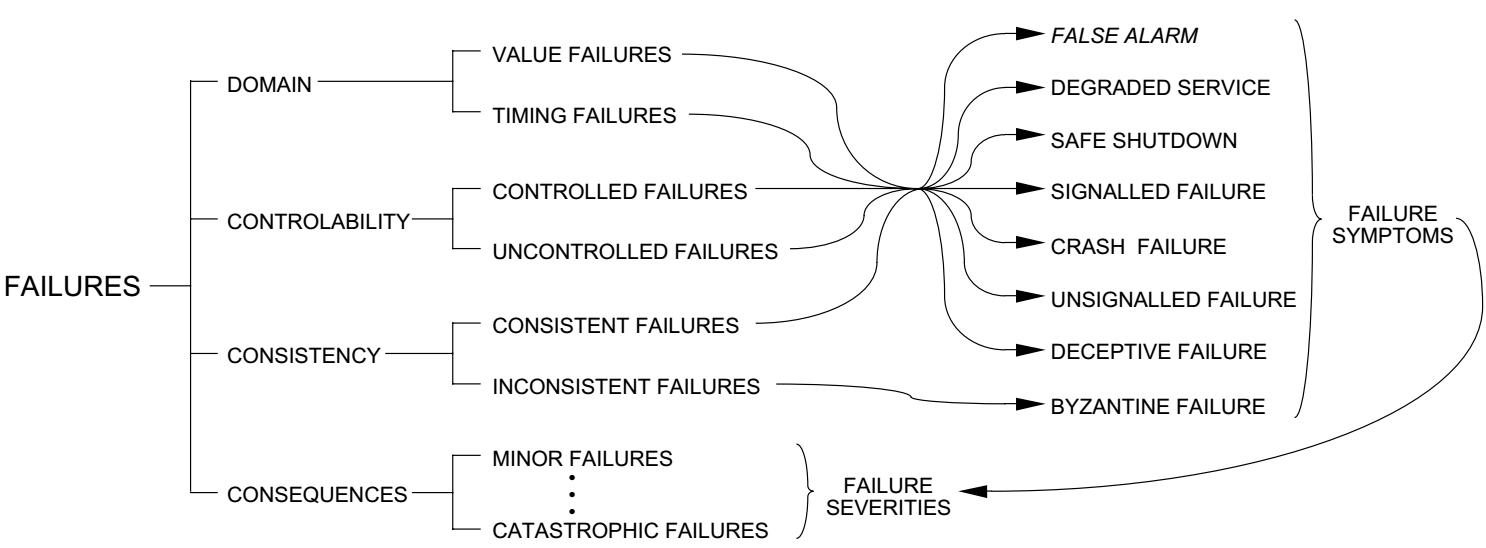
\includegraphics[width=0.7\linewidth]{concepts_fail}
\caption{Failure Modes}
\label{fig:concepts_fail}
\end{figure}

\begin{figure}
\centering
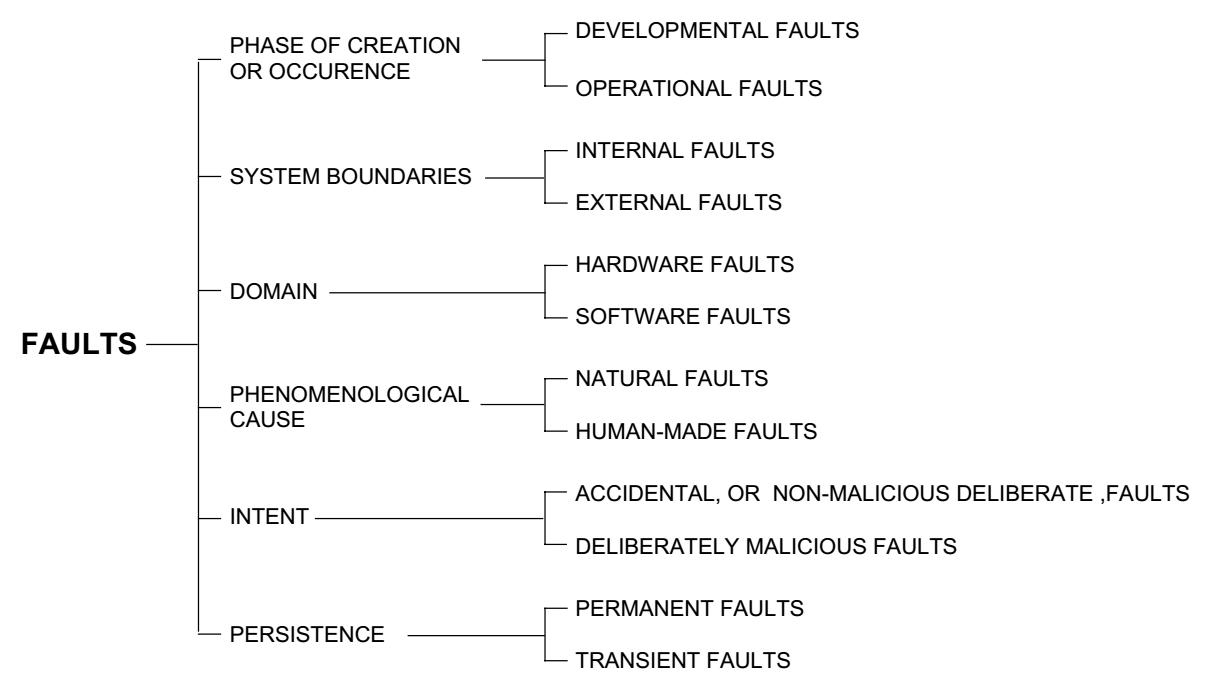
\includegraphics[width=0.7\linewidth]{concepts_fault}
\caption{Fault Classes}
\label{fig:concepts_fault}
\end{figure}

\section{Means}

\subsection{Fault Prevention}

Fault prevention requires quality control techniques employed during the design and manufacturing of the system.
That includes, e.g., structured programming, information hiding, or modularization.

Shielding, radiation hardening, etc., are needed to to prevent physical faults.
Training and maintenance procedures aim at preventing interaction faults.
Firewalls and similar defenses intend to prevent malicious faults.

\subsection{Fault Tolerance}

Fault tolerance is intended to preserve the delivery of correct service in the presence of active faults.
This may refer to accidental or malicious faults.

\paragraph{Error detection}
An error that is present but not detected is a \textbf{latent} error. 
Concurrent error detection takes place during service delivery.
Preemptive error detection takes place while service delivery is suspended; it checks the
system for latent errors and dormant faults.

\paragraph{Recovery}
Recovery consists of error handling and fault handling.

Error handling eliminates errors from the system state by
\begin{compactitem}
  \item rollback: the state is transformed to a previously saved state
  \item compensation: the erroneous state is redundant enough to eliminate the error,
  \item rollforward: the state is transformed to a new state without the detected error.
\end{compactitem}

Fault handling prevents located faults from being activated again by
\begin{compactitem}
  \item fault diagnosis: identify location and type of the cause of an error
  \item fault isolation: exclude the fault form future service delivery, i.e., make the fault dormant
  \item system reconfiguration: switch to non-failed components
  \item system reinitialization: update to a new configuration of the system
\end{compactitem}

The choice of error detection, error handling, and fault handling techniques, and of their implementation, is directly related to the underlying fault assumption.

Fault tolerance is recursive: Its implementation must be protected against faults as well.


\subsection{Fault Removal}

\paragraph{Development Phase}
Fault removal during the development phase of a system consists of three steps:
\begin{compactitem}
 \item Verification checks whether the system satisfies required properties.
 \item If verification fails, diagnosis identifies the faults that prevented verification.
 \item After diagnosis, correction is carried, and verification repeated.
\end{compactitem}

Multiple different properties can be verified:
\begin{compactitem}
 \item Verifying the specification is usually referred to as validation.
Static verification does not exercise the systems and uses static analysis (e.g., inspections or walk-through), model-checking, or theorem proving.
Dynamic verification exercises the systems and uses testing.
\item Verifying the fault tolerance mechanism.
This can employ formal static verification or fault injection, i.e., testing where intentional faults or errors are part of the test.
\item Verifying that the system cannot do more than specified is especially relevant for safety and security.
\end{compactitem}

\emph{Design for verifiability} means to design a system in such a way that verification becomes easy.

\paragraph{Operation Phase}
Fault removal during the life time of a systems employs two methods:
\begin{compactitem}
\item Corrective maintenance removes faults that have produced errors that were detected and reported.
\item Preventive maintenance uncovers faults before they cause errors.
This may also include design faults that have caused errors in similar systems.
\end{compactitem}

Fault removal during operation often first isolates the fault (e.g., by a workaround or patch) before the actual removal is carried out.

\subsection{Fault Forecasting}

Fault forecasting evaluates a system with respect to fault occurrence or activation.
It has two aspects:
\begin{compactitem}
  \item Qualitative evaluation identifies, classifies, and ranks the failure modes, or the event combinations that would lead to system failures.
  \item Quantitative evaluation determines the probabilities to which some of the attributes of dependability are satisfied, which are then viewed as measures of dependability.
  This may use, e.g., Markov chains or Petri nets.
\end{compactitem}

%Dependability can remain stable, grow, or decrease during a system's life-cycle.
%These can be measure by failure intensity, i.e., the number of failures per unit of time.
%It typically first decreases, then stabilizes, then increases, and the cycle resumes.
%
%The alternation of correct-incorrect service delivery is quantified to define reliability, availability, and maintainability as measures of dependability:
%\begin{compactitem}
% \item reliability: a measure of the continuous delivery of correct service---or, equivalently, of the time to failure,
% \item availability: a measure of the delivery of correct service with respect to the alternation of correct and incorrect service,
%• maintainability: a measure of the time to service restoration since the last failure occurrence, or
%equivalently, measure of the continuous delivery of incorrect service,
%• safety is an extension of reliability: when the state of correct service and the states of incorrect
%service due to non-catastrophic failure are grouped into a safe state (in the sense of being free from
%catastrophic damage, not from danger), safety is a measure of continuous safeness, or equivalently,
%of the time to catastrophic failure; safety is thus reliability with respect to catastrophic failures.
%Generally, a system delivers several services, and there often are two or more modes of service quality,
%e.g. ranging from full capacity to emergency service. These modes distinguish less and less complete
%service deliveries. Performance-related measures of dependability are usually subsumed into the notion
%of performability.

%The main approaches to derive probabilistic measures of dependability measures are modeling and testing.
%These approaches are complementary since modeling needs data on the basic processes modeled (failure process, maintenance process, system activation process, etc.), that may be obtained either by testing, or by the processing of failure data.
%When evaluating fault-tolerant systems, the effectiveness of error and fault handling mechanisms, i.e., their coverage, has a drastic influence on dependability measures.
%The evaluation of coverage can be performed either through modeling or through testing, i.e. fault injection.